\section{Rumore nello stack}

In questo libro si fa spesso riferimento a \q{rumore} o \q{spazzatura} (garbage) nello stack o in memoria.

Da dove arrivano?
Sono cio' che resta dopo l'esecuzione di altre funzioni.
Un piccolo esempio:

\lstinputlisting{patterns/02_stack/08_noise/st.c}

Compilando si ottiene:

\lstinputlisting[caption=\NonOptimizing MSVC 2010]{patterns/02_stack/08_noise/st.asm}

Il compilatore si lamentera' un pochino\dots

\begin{lstlisting}
c:\Polygon\c>cl st.c /Fast.asm /MD
Microsoft (R) 32-bit C/C++ Optimizing Compiler Version 16.00.40219.01 for 80x86
Copyright (C) Microsoft Corporation.  All rights reserved.

st.c
c:\polygon\c\st.c(11) : warning C4700: uninitialized local variable 'c' used
c:\polygon\c\st.c(11) : warning C4700: uninitialized local variable 'b' used
c:\polygon\c\st.c(11) : warning C4700: uninitialized local variable 'a' used
Microsoft (R) Incremental Linker Version 10.00.40219.01
Copyright (C) Microsoft Corporation.  All rights reserved.

/out:st.exe
st.obj
\end{lstlisting}

Ma quando avvieremo il programma \dots

\begin{lstlisting}
c:\Polygon\c>st
1, 2, 3
\end{lstlisting}

Oh, che cosa strana! Non abbiamo impostato il valore di alcuna variabile in \TT{f2()}. 
Si tratta di valori \q{fantasma} , che si trovano ancora nello stack.

\clearpage
Carichiamo l'esempio in \olly:

\begin{figure}[H]
\centering
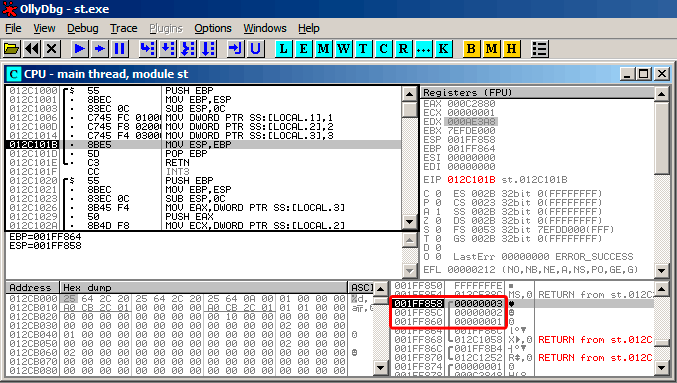
\includegraphics[scale=\FigScale]{patterns/02_stack/08_noise/olly1.png}
\caption{\olly: \TT{f1()}}
\label{fig:stack_noise_olly1}
\end{figure}

Quando \TT{f1()} assegna le variabili $a$, $b$ e $c$, i loro valori sono memorizzati all'indirizzo \TT{0x1FF860} e seguenti.

\clearpage
E quando viene eseguita \TT{f2()}:

\begin{figure}[H]
\centering
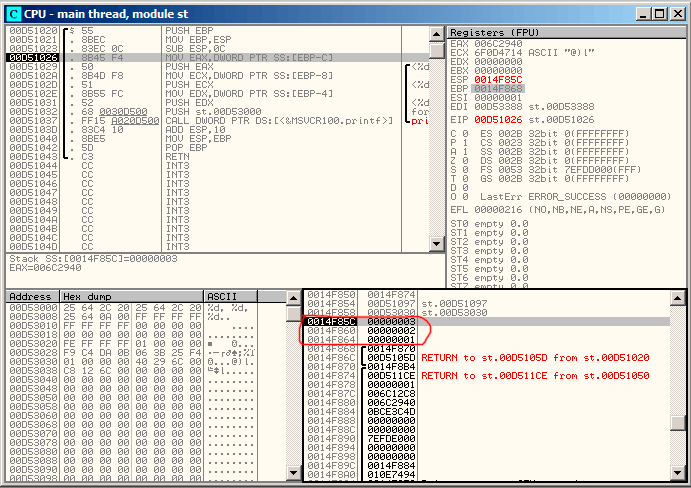
\includegraphics[scale=\FigScale]{patterns/02_stack/08_noise/olly2.png}
\caption{\olly: \TT{f2()}}
\label{fig:stack_noise_olly2}
\end{figure}

... $a$, $b$ e $c$ di \TT{f2()} si trovano agli stessi indirizzi!
Nessuno ha ancora sovrascritto quei valori, e a quel punto restano intatti.
Quindi, affinche' questa strana situazione si verifichi, piu' funzioni devono essere chiamate una dopo l'altra e
\ac{SP} deve essere uguale ad ogni ingresso nella funzione (ovvero le funzioni devono avere lo stesso numero di argomenti).
A quel punto le variabili locali si troveranno nelle stesse posizioni nello stack.
Per riassumere, tutti i valori nello stack (e nelle celle di memoria in generale) hanno valori lasciati li' dall'esecuzione di funzioni precedenti.
Non sono letteralmente randomici, piuttosto hanno valori non predicibili.
C'e' un'altra opzione?
Sarebbe possibile ripulire porzioni dello stack prima di ogni esecuzione di una funzione, ma sarebbe un lavoro extra inutile.

\subsection{MSVC 2013}

L'esempio e' stato compilato con MSVC 2010.
Un lettore di questo libro ha provato a compilare l'esempio con MSVC 2013, lo ha eseguito, ed ha ottenuto i 3 numeri in ordine inverso:%

\begin{lstlisting}
c:\Polygon\c>st
3, 2, 1
\end{lstlisting}

Perche'?
Ho compilato anche io l'esempio in MSVC 2013 ed ho visto questo:


\begin{lstlisting}[caption=MSVC 2013]
_a$ = -12						; size = 4
_b$ = -8						; size = 4
_c$ = -4						; size = 4
_f2	PROC

...

_f2	ENDP

_c$ = -12						; size = 4
_b$ = -8						; size = 4
_a$ = -4						; size = 4
_f1	PROC

...

_f1	ENDP
\end{lstlisting}

Contrariamente a MSVC 2010, MSVC 2013 ha allocato le variabili a/b/c nella funzione \TT{f2()} in ordine inverso.%
E cio' e' del tutto corretto, perche' lo standard \CCpp non ha una regola che definisce in quale ordine le variabili locali devono essere allocate nello stack.
La ragione per cui si presenta questa differenza e' che MSVC 2010 ha un solo modo per farlo, mentre MSVC 2013 ha probabilmente subito modifiche all'interno del compilatore, e si comporta quindi in modo leggermente diverso. 
